Let $\vec{x}$ be the point on y-axis.Then
\begin{equation}
   \vec{x}= y\myvec{0\\1}= y \vec{e}_2
\end{equation}
and from the given information,
\begin{align}
\norm{\vec{x}-\vec{A}}^2 &=\norm{\vec{x}-\vec{B}}^2 
\\
 \label{aug/2/25/eq:2}
2 \vec{x}(\vec{A}-\vec{B})^{\top}&=\norm{\vec{A}}^2-\norm{\vec{B}}^2
\\
\text{or, }
 2y\vec{e}_2(\vec{A}^{\top}-\vec{B}^{\top})&=\norm{\vec{A}}^2-\norm{\vec{B}}^2\\
 \implies \vec{y} &= \frac{\norm{\vec{A}}^2 - \norm{\vec{B}}^2}{2\vec{e}_2(\vec{A}-\vec{B})^{\top}}\\
 &= 9
\end{align}
upon substituting numerical values.
%     
This is verified in Fig. \ref{aug/2/25/Graphical solution}

\begin{figure}[ht]
    \centering
    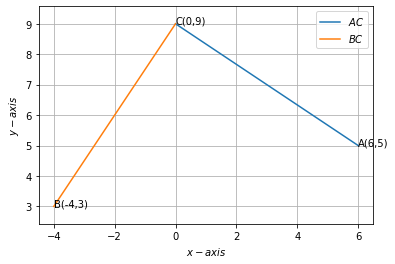
\includegraphics[width=\columnwidth]{solutions/july/25/download.png}
    \caption{}
    \label{aug/2/25/Graphical solution}
\end{figure}